\chapter{A Interface e sua ligação com IoT}
\label{chapter:interface_iot}

No capítulo \ref{chapter:industria_4_0_iot}, foi visto as bases para se implementar um projeto de IoT. A área começou a receber fortes investimentos e atenção por volta de 2009 e desde então foram feitas consideráveis implementações utilizando tecnologias e protocolos diferentes. Neste capítulo serão apresentados algumas dessas variações, para fins de comparação e respaldo para importância e objetivo deste projeto.

\section{Tecnologias em IoT}
\label{section:tecnologias_iot}

Estas são algumas tecnologias que satisfazem as condições apresentadas para um sistema IoT, nem todas utilizam o protocolo TCP/IP, mas todas são  capazes de fazer seus dispositivos comunicarem-se em tempo real levando em consideração seus alcances e escalabilidade.

As primeiras aplicações de IoT foram em laboratórios de aplicações de RFID \cite{Rampim:iot}, junto com códigos bidimensionais, para aplicações de identificação de objetos. Uma das soluções mais populares e de baixo custo de IoT utilizando Rádio frequência.

Redes que utilizam bandas restritas visando baixo consumo e distância de transmissão são a nova fronteira, as mensagens de IoT são geralmente curtas, dados telemétricos, status etc, logo estes protocolos mostram-se úteis para este tipo de aplicação. Já se encontram implementadas algumas redes como SigFox \cite{Sigfox} e LoRa \cite{LoRa}. 

As novas gerações de Bluetooth consomem muito menos energia, o que tornaram a tecnologia viável para aplicações IoT. Geralmente, módulos Bluetooth são utilizados como beacons \cite{Endeavor:Beacons}. Pontos espalhados por uma região, no qual podem se comunicar com os módulos de dispositivos mobile ao se aproximar, oferecendo links para conteúdo e exclusividades.

As tecnologias mais comuns de se encontrar em aplicações IoT, os protocolos construídos com base no TCP/IP são vastamente utilizados e possuem uma rede mundialmente distribuída, o que facilita o uso. Pode-se implementar uma gama de protocolos de aplicações, alguns mais eficientes que outros.

O protocolo mais simples seria o HTTP, altamente usado na internet, porém não é eficiente no consumo de energia por abrir uma conexão a cada envio de dados. Para minimizar estas desvantagens, foi desenvolvido o CoAP \cite{coap} protocolo nos mesmos moldes do HTTP com o modelo REST, porém mais simples, mais leve, com baixo overhead e utilizado em redes locais.

Mas os mais utilizados em aplicações são sem dúvidas os protocolos que mantém conexão aberta, em especial Websocket e MQTT, sendo o primeiro mais utilizado para chats e mensagens e o segundo domina o mundo do M2M e Telemetria.


\section{A Interface}
\label{section:interface}

Inicialmente, os conceitos e ideias do projeto eram voltados a desenvolver uma interface no qual um desenvolvedor poderia implementar um sistema IoT de ponta a ponta utilizando APIs que direcionariam para um desses protocolos da seção \ref{section:tecnologias_iot}, porém as diferenças entre os protocolos e as camadas de base, fazem com que esta solução esteja mais distante. Então o foco voltou-se  para tecnologias que tenham base na pilha TCP/IP, por sua vasta implementação nas redes industriais e residências e na Internet.

Neste projeto iremos ver a implementação desta interface para o protocolo MQTT, cuja escolha será justificada adiante. Serão descritas as interfaces para as três camadas, que são de baixo custo, open-source e altamente escaláveis para construir outras aplicações com esta como base.
 
Para abstrair as camadas e aplicação, a interface deve estar dentro dos requisitos do IoT, bem assim como apresentar uma estrutura que se traduza aos protocolos baseados TCP/IP, para isso, algumas características fundamentais podem ser destacadas como base para um sistema IoT descritos.

\begin{itemize}

\item Full-Duplex. Capaz de receber e enviar mensagens ao mesmo tempo;
\item Multicast. Capaz de enviar mensagens um ou mais dispositivos simultâneos;
\item Envio de mensagens em tempo real;

\end{itemize}


\begin{figure}[h!]
\centering
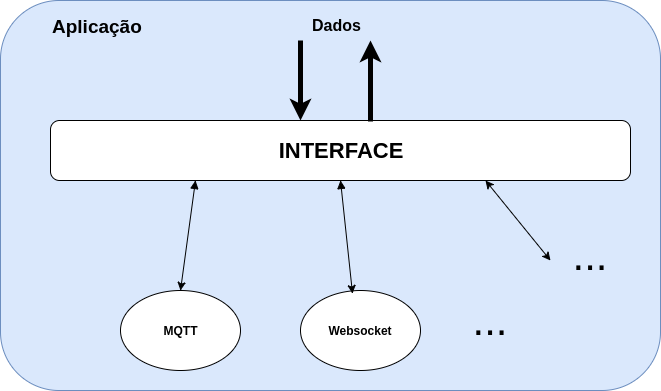
\includegraphics[width=12cm]{./02_Capitulos/02_Cap2/figures/camada_abstracao}
\caption{Interface de comunicação. A interface tem seu próprio protocolo que direciona e se comunica a um ou mais protocolos de aplicação}
\label{fig:2.2.0/camada_abatracao}
\end{figure}

Essas características estão dentro do escopo apresentado no capítulo \ref{chapter:industria_4_0_iot}, a estratégia foi direcionada para protocolos que atendessem esse pré-requisito, assim construindo uma camada de abstração da interface por cima dos protocolos que contemplam essas características como mostra a figure \ref{fig:2.2.0/camada_abatracao}, o que será mais detalhado no próximo capítulo.


